\section{The True Man}

\begin{quotex}
Then God said, ``Let us make man in our image, after our likeness; and let them have dominion over the fish of the sea, and over the birds of the air, and over the cattle, and over all the earth, and over every creeping thing that creeps upon the earth." So God created man in His own image, in the image of God He created him; male and female He created them. And God blessed them, and God said to them, ``Be fruitful and multiply, and fill the earth and subdue it; and have dominion over the fish of the sea and over the birds of the air and over every living thing that moves upon the earth." 

\end{quotex}

In \emph{The Great Triad}, \textbf{Rene Guenon} describes the \textbf{True Man} as the being who has actualized all his possibilities as a man. True Man is also man as he is in the \textbf{Primordial State}, in contrast to the ``ordinary man" or today. Using the initiatic formula ``\emph{Heaven is his father, earth is his mother}", man can be described as the \textbf{Son of Heaven and Earth}, thus is the third term of that triad. The schema in Table~\ref{tab:ManPrinciples} relates this symbolism to various Traditions:

\begin{table}[h]\small
\begin{tabularx}{\textwidth}{*6{X}}\toprule
Masculine Principle &
Heaven &
Essence &
Yang &
Actuality &
Interior\\\midrule
Feminine Principle &
Earth &
Substance &
Yin &
Potency &
Exterior\\\bottomrule
\end{tabularx}
\label{tab:ManPrinciples}
\caption{Man Principles}
\end{table}
Although everything has aspects of both principles, True Man has them in a balanced way. He ``possesses the fullness of human nature, for he has developed in himself the totality of possibilities that implies." For examples of what this may mean, see \textit{Cagliostro the Trickster}\footnote{\url{https://gornahoor.net/?p=764}}, \textit{Genius and the Real Man}\footnote{See Section \ref{sec:GeniusRealMan} in this book.}, \textit{Life of a Contemporary Hermetist}\footnote{\url{https://gornahoor.net/?p=793}}, or \textit{The Wise Man rules the Elements}\footnote{\url{https://gornahoor.net/?p=1010}}. 

Ordinary man, on the other hand, has developed primarily at the corporeal or hylic level, and is thus yin, or passive, in relation to the Cosmos. As Evola writes of this type: 

\begin{quotex}
the ``I" still lives only as if in a dream: it is not yet a self-consciousness, nor an autonomous principle of action: immersed in an immediate, indistinct coalescence with nature and the world, we can say that it is not so much he who thinks, speaks, and asserts himself, as much as that various forces and impulses think, speak and assert themselves in him. He therefore is only a type of medium, a passive instrument that has his very life outside himself, and he experiences everything as grace, as spontaneity, as the immediate self-manifestation of something that transcends him. (From \emph{The Individual and the Becoming of the World}.) 

\end{quotex}
The ordinary man is described as the Son of the Earth. For the true man, his actuality is equal to his potency, that is, he is perfectly balanced between \emph{yin} and \emph{yang}. He is thus \emph{yang}, or active, in relation to the Cosmos, because celestial nature is predominant over terrestrial nature; he therefore is in the \emph{center}.

\begin{wrapfigure}{rt}{.4\textwidth}
 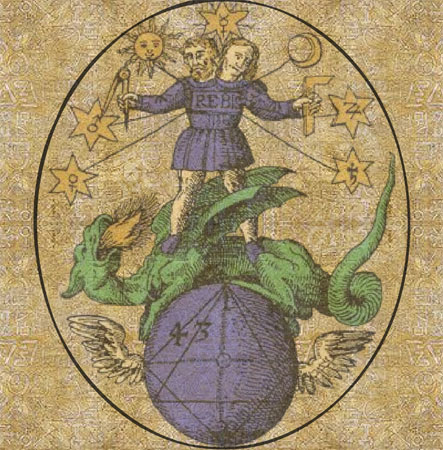
\includegraphics[scale=.3]{a20100921TheTrueMan-img001.jpg}
 \end{wrapfigure}

The fall of the True Man from the Primordial State is the result of a decentering, a change in consciousness to exteriority from interiority. Now the Primordial State is the \textbf{Androgyne} of the Alchemists, that is, the perfect balance of the male and female principles. From the center, he is the unmoved mover, and his actions are \emph{wei wu wei}, or non-acting activity.

We see that the shift from the ordinary state to the Primordial State represents, spiritually, a transition from a passive, \emph{yin}, or feminine state of existence to a more active, \emph{yang}, or masculine state. This is the opposite of the ``macho" man, obsessed with frenetic activity for its own sake and focused solely on material life. Yet, when esoteric teachings enter into the popular domain, they are completely misunderstood by those at the hylic and psychic level. When such types hear of the Androgyne, they can only envision a feminization of man, that is, a exterior type of man taking on more effeminate characteristics. Thus the \emph{epicene} man of today, common in the West, regards himself \emph{ipso facto} as an advanced spiritual being. Unfortunately, this occludes the true spiritual nature of man and discourages many more masculine men from developing themselves in that direction.



\flrightit{Posted on 2010-09-21 by Cologero }

\begin{center}* * *\end{center}

\begin{footnotesize}\begin{sffamily}



\texttt{James O'Meara on 2010-09-21 at 21:33 said: }

The `androgyne' is not a hapax legomenon in Evola's work, but occurs time and again. It's all well to say, ``Well, of course, he's not talking about, well, you know…" But if not, then what on Earth IS he talking about? 

Of course, words like `epicene' are culturally determined. I think `Alan Alda' and of course that kind of ``sensitive liberal man" would be loathed by Evola. Funny thing is: look at Evola's passport photo, for example: fancy suit, monocle. He's a FAG by today's standards, determined as they are by the rise of the telluric negro [Evola's definitive essay on `America Negrified’].

Childless, never married. Hmmm. Mighty suspicious if he were, say, running for Congress. And what would the judaic-inspired ``family values" crowd think of his mockery of marriage and population growth in Men Among the Ruins or Ride the Tiger?

Here is what E. says in ``Serpentine Wisdom" [i.e., Taoism], after describing the Man of Tao who `acts without acting' etc.:

``How disheartening to those who uphold the myth of manhood based on muscles and metallic strength: this alone is the TRUE man, the ABSOLUTE man. He [Evola's ideal] absorbs within himself the ambiguous virtue of the female…. `The Way that is the Way is not the ordinary way' indeed…"

In The Hermetic Tradition, Evola expands on the idea as involving a becoming female [Hercules in drag], as it were coming under the domination of the Woman as a necessary stage; the salient point is, does one remain so, or does one conquer the female [the Hermetic Incest]and thus acquire her unique powers for oneself. 

Now, does that make a difference or not? 

If you look at popular culture, it's clear that the `fag' is not just the simpering queen, or Alan Alda, but also any White man acting in the light of the Aryan ideal. Dressing well, speaking correctly, acting modestly, well read. The average ``Traditionalist," reading books and even knowing several languages, is clearly a fag. 

To the extent that a culture, like America, takes the Negro as the Ideal Man, then that ideal will be psychic, even material; and vice versa, the causality is not important here.

To the extent that a culture adheres to Aryan ideal, rooted in the primitive Mannerbund, then it will not be a culture that idealizes the brute, but the warrior, Greek or Icelandic, who triumphs in battle and then spontaneously recites poetry. Long blonde hair flowing, he will more closely resemble Leif Garrett than Puff Daddy. Pausanias, not Alcibiades or Themistocles.


\hfill

\texttt{Matt on 2010-09-22 at 01:37 said: }

James,

Those are some good points. I think Evola would say that what people think of today as true masculinity would fit his description of what he called titanic masculinity, the low/crude form of masculinity, in contrast to Apollonian masculinity (high form of masculinity), which has some attributes (that you mentioned) that wouldn't be considered very masculine in modern society.


\hfill

\texttt{James O'Meara on 2010-09-22 at 09:59 said: }

Thanks, Matt. `Titanic' may be the word. Speaking of ``low/crude," on my blog I have frequently observed that, in terms of popular music, when White music dominated [from Folk to Southern Rock to Heavy Metal] the performers chose to appear, and were highly successful in, ways that would be considered entirely `gay' today; now that the Negro is the ideal, the ideal is indeed the low, crude, violent thug. 

In terms of civilization, was not the Titanic a stage where men rebelled against an oppressive Amazonian rule, and ruled with a resulting crude and unrefined idea of masculinity? Similar, in the regression of the castes, to the crude rule of the Khshatrias after the Priest/King rule was split and Priest [feminine, passive] had ruled alone first? The Priest/King is the original Androgyne.


\hfill

\texttt{Cologero on 2010-09-22 at 23:43 said: }

The point is that the True Man is a metaphysical concept, not a particular historical or empirical type of man. That is looking at things from the exterior, whereas we are concerned with interiority. In the Hermetic Tradition, Evola gives some examples (ch 30):

``a great physical and intellectual equilibrium, … a healthy body without appetites or desires, being at peace with oneself and others; making oneself absolute master of the animal envelope in order to make of it an obedient servant …"

This is the point again: yang gaining control over yin.

Again, referring to Eliphas Levi, Evola writes:

``we must rid the will of any dependency and accustom it to domination; we must become absolute master of the self, learn to deny the call of pleasusre, hunger and sleep and be unmoved by success or failure." and then ``…submit in every organ to the spirit"

What a True Man looks like, what he does, or how he acts will not reveal his inner state to the vulgar. Having actualized all his potentials, he is free to act in any way suitable to his purposed in every situation.


\hfill

\texttt{James O'Meara on 2010-09-23 at 08:43 said: }

Indeed. The True Man would be master of appearances, and perhaps, as E. says regarding The Mage and the Taoist Masters, he may prefer not to appear at all!


\hfill

\texttt{Cologero on 2010-09-24 at 14:02 said: }

Apparently Guenon's concept is not clear when he writes that the True Man has actualized all his possibilities. That means that the world of appearances (yin or the feminine) is under the domination of the True Man as yang. In the Triad, Man is the mediator between Heaven and Earth … the task of the True Man is to bring the ideas or Essences into manifestation … that is a demonstration of Power.


\hfill

\texttt{James O'Meara on 2010-09-24 at 18:51 said: }

Speaking of the Path of Cinnabar, we learn there how Evola passed from philosopher of the Absolute Ego to Guenonian Traditionalism by realizing that if the True Will needed to be ``embodied" in concrete history it could take the form of the founders of the various traditions. Now clearly all these traditions are very different in appearance; in the same way, all True Men are in some sense not only similar but the same man, transcendentally, but manifest in different forms, by their Absolute Will.


\hfill

\texttt{Cologero on 2010-09-29 at 00:17 said: }

A similar take on this issue from a rather different perspective:

Etiquette and Protocol are Manly Pursuits

\url{http://rencesvals.blogspot.com/2010/09/etiquette-and-protocol-are-manly.html}


\hfill

\texttt{James O'Meara on 2010-09-30 at 15:52 said: }

Well, if we are recomeneding books, how about Hagakure: The Book of the Samurai? Found a copy for a buck yesterday, athough I already have Mishima's essay on it. A random reviewer at Amazon makes a point that might relate to how the True Man functions:

``[T]his book is not a rigorous philosophical treatise, at least not in the way that Western scholars would define it. Instead, it is a collection of stories and phrases about a certain way of living. It doesn't hold up to scientific cross-examination (the author contradicts himself frequently), but it shouldn't have to. Yamamoto gives the impression that if faced with a philosophical attack on his ``way", he would shrug his shoulders and say, ``Yes, but that doesn't change a thing." In other words, his examples and aphorisms speak for themselves, and are not meant to either exclude other points of view or force others into conformity. Yamamoto even states that the Way he advocates is specific to his region of Japan — samurai of neighboring regions are free to develop their own Ways."


\hfill

\texttt{Ernest on 2010-09-30 at 18:27 said: }

Also from the Hagakure:

``It is said that what is called the Spirit of an Age is something to which one cannot return. That this spirit gradually dissipates is due to the world's coming to an end.
In the same way, a single year does not have just spring or summer. A single day, too, is the same. For this reason, although one would like to change today's world back to the spirit of one hundred years or more ago, it cannot be done. Thus it is important to make the best out of every generation."

And on the subject of Real/True Men:

``According to a certain person, a number of years ago Matsuguma Kyoan told this story: In the practice of medicine there is a differentiation of treatment according to the Yin and Yang of men and women. There is also a difference in pulse. In the last fifty years, however, men's pulse has become the same as women's. Noticing this, in the treatment of eye disease I applied women's treatment to men and found it suitable. When I observed the application of men's treatment to men, there was no result. Thus I knew that men's spirit had weakened and that they had become the same as women, and the end of the world had come. Since I witnessed this with certainty, I kept it a secret.

When looking at the men of today with this in mind, those who could be thought to have a woman's pulse are many indeed, and those who seem like real men few. Because of this, if one were to make a little effort, he would be able to take the upper hand quite easily."


\hfill

\texttt{James O'Meara on 2010-10-01 at 10:22 said: }

Indeed, such womanish men would not make suitable lovers for the samurai. This brings us back to the our topic; the True Man is not socially determined. Indeed, in today's materialistic and quantitative Western world, ``no one seems to tell young men the `musts' of shudo [``The Way of Men, meaning homosexuality, which was rampant in that era" as the translator helpfully explains]I.180, while the Judeo-Christian ideal of the Family Values Man reigns supreme.


\end{sffamily}\end{footnotesize}
